\chapter{Frontend}

This chapter describes the frontend of SableWasm. The front end consists of two parts, the bytecode parser and validation pass.  WebAssembly is a continuously evolving language, and its community might add new instructions in the future. Hence, the parser and the bytecode validation phase's design closely follow WebAssembly's specification and modular to ensure the framework's extensibility. A read-only view of the module structure provides additional functionality. The parser and validation phase design focuses on performance, both in execution time and memory footprint. 

\section{Bytecode Parser}
One of WebAssembly's binary format design goals is simple to parse. Although there are existing open-source bytecode parsing and validation library available when writing the thesis, such as WABT \footnote{WebAssembly Binary Toolkit: \url{https://github.com/WebAssembly/wabt.git}} provided by the WebAssembly community, there is no suitable library at the time when the project starts. Thus, for SableWasm, we implement our bytecode parsing frontend instead. The bytecode parser consists of three components, byte-source reader, WebAssembly bytecode parser and parser delegate. This section will give a brief description of each component, and figure~\ref{fig:sablewasm-parser} presents a general illustration of the parser's design.  

\begin{figure}
  \centering
  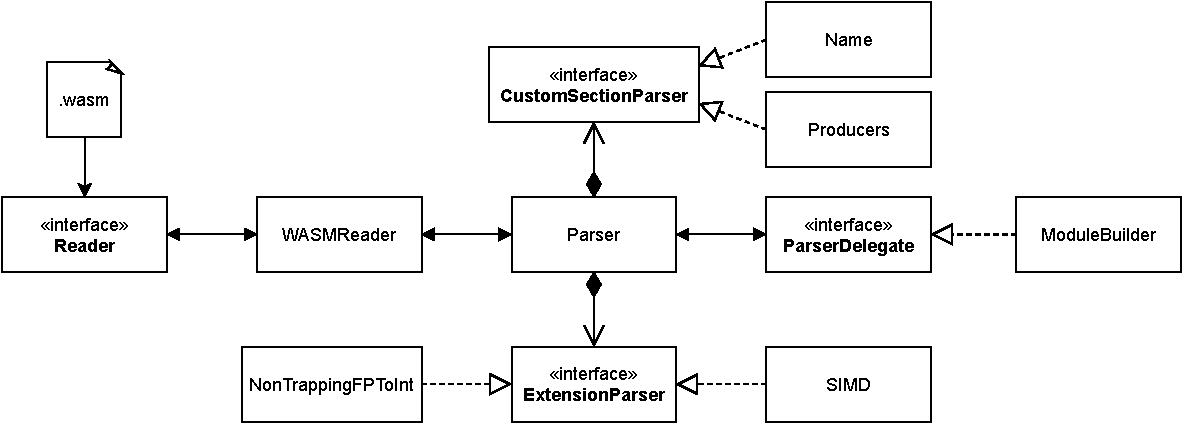
\includegraphics[width=\textwidth]{Images/sablewasm-parser.pdf}
  \caption{SableWasm parser}
  \label{fig:sablewasm-parser}
\end{figure}

\paragraph{Byte-source Reader}
The byte-source reader consists of two parts, a byte-buffer reader and a WebAssmebly reader. The byte-buffer reader provides essential functionalities such as read and skips. Additionally, the byte-buffer reader also needs to support rewind and barrier. Any out of bound access, either beyond the barrier or byte stream exhausted, the byte-buffer reader will signal via exceptions. On the other hand, the WebAssembly reader provides a richer interface to the parser, such as decode LEB-128 encoded integers and parsing WebAssembly value types. The WebAssembly reader is also responsible for validating the result before passing it to the parser. In the case the result is invalid, the reader throws exceptions similar to the byte-buffer reader.

\paragraph{WebAssembly Parser}
WebAssembly parser is the kernel part of the parsing framework. As we discussed earlier in the chapter, one of the primary design goals of the framework is its extensibility. Hence, the SableWasm parser is modular and consists of three parts, parser core, custom section parser and instruction extension parser. The grammar for WebAssembly binary representation is quite simple, and therefore, the parser core implements a simple top-down recursive descent parser with a single byte look-ahead.

\emph{Custom sections} are a special section defined in the WebAssembly standard. They are essentially a binary data chunk tagged with a string name. How to interpret the binary data is different from one to another. These custom sections can either be standardized by the community or defined specific to a toolchain. In this project, we implement two custom sections standardized by the WebAssembly working group, namely \emph{Name} section and \emph{Producer} section. The \emph{Name} section gives human-readable names to functions and their local variables that help program debugging. The specification does not require these names to be the same as the import or export names. There is no direct support for more detailed debug information encoding in WebAssembly, at the time of thesis writing. However, extensions are working on this problem, such as DWARF for WebAssembly \footnote{DWARF for WebAssembly: \url{https://yurydelendik.github.io/webassembly-dwarf/}}; on the other hand, the \emph{Producer} section is relatively simple. It only encodes the information about the toolchain that generates the module, such as the toolchain name and version. All custom section parsers in SableWasm derived from the base class \texttt{CustomSection}. The parser core will dispatch the binary chunk to search custom section parser based on the name tag. Each custom section parser manages its results and does not communicate to the parser delegate directly. 

Instruction extension parsers focus on another different aspect of the WebAssembly module. In the background section, we have visited several extensions that merged to the WebAssembly specification. A quick reminder, WebAssembly extensions can insert or modify the instructions defined in the minimum-viable-product (MVP)  specification. The SableWasm WebAssembly parser employs instruction extension parsers to address this problem. When the parser intends to parse an instruction, it will iterate over all its instruction extension parsers in a chained manner. If the instruction opcode is not recognized by any registered instruction extension parser nor in the minimum-viable-product specification, the parser will signal the error by throwing an exception. An instruction extension parser can also override the default behaviour for MVP instructions by handling the instruction early, though, in the current version of WebAssembly, no extensions modify the semantics of these instructions. In this project, we implement two instruction extension parsers, the Non-trapping-float-to-int conversion parser and SIMD parser, which handles the instructions introduced by the extensions as their names suggest.

\paragraph{Parser Delegate}
The last part of the SableWasm WebAssembly bytecode parser is the parser delegate. The parser delegate and parser are direct implementations of the common delegation patterns seen in many other projects, separating the parsing from the heavy lifting of module construction. One can implement a validation pass at this level without module construction. However, in this project, we implement our bytecode validation pass after the module construction, giving space for further projects focusing on bytecode-level transformation. We will discuss the implementation of such validation pass later in the chapter. 

In this section, we give a brief overview of the parser framework introduced in the SableWasm. In the next section, we will discuss the WebAssembly bytecode representation used in the project and several techniques to improve the performance and ensure flexibility.

\section{WebAssembly Bytecode Representation}

\begin{figure}
  \centering
  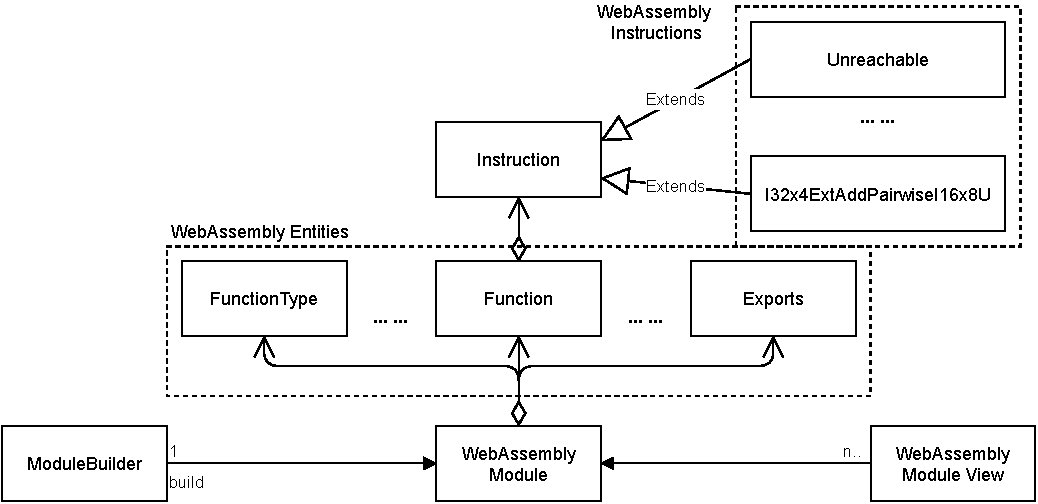
\includegraphics[width=\textwidth]{Images/sablewasm-bytecode.pdf}
  \caption{SableWasm bytecode representation}
  \label{fig:sablewasm-bytecode}
\end{figure}

WebAssembly specification provides compact representations in both binary and text formats \cite{10.1145/3062341.3062363}, and these specifications might subject to change in the future. In SableWasm, we implement our bytecode representation as close to the specification as possible.  Hence, in the future, if the community alters the specification in the future, we can apply fixes to the bytecode representation in a straightforward manner without introducing extra complexity. In figure~\ref{fig:sablewasm-bytecode}, we present an illustration of the bytecode representation used in SableWasm. Compare to the representation given in the WebAssembly specification, the only difference we have is the function section. The standard WebAssembly bytecode representation actually splits the function section into two different sections, namely \emph{function} and \emph{code}, to achieve its one-pass validation goal. The \emph{function} section contains the type of all functions defined in the module, serving similar to function declarations in other languages. Later in the module, \emph{code} section defines them. On the other hand, in SableWasm, we merge these two sections into a single function section. A function in SableWasm bytecode representation contains both its type and its definition.

\paragraph{WebAssmebly Module View}
The WebAssembly module structure only serves as a storage container for the bytecode representation and itself does not provide an interface to the user, except retrieving entities by index. Additionally, WebAssembly standard binary format focuses more on compactness instead of usability, which leads to complexity when retrieving the information. For example, to avoid duplication, the function types are stored in their section, namely, \emph{type} section. Later in the module, any reference to the type becomes an indices respect to this section. Another example is entity indices. WebAssembly specification requires that every import entry in the \emph{import} section implicitly introduces an index in its corresponding class. These indices should come before any definition introduced in the module. These two rules suggest that to retrieve an entity by index, one should first iterate over all the imports and then locate the entity accordingly, which is a relatively expansive operation. To address these problems, we implement a read-only view of the WebAssembly module that cache the indices and provides additional features. 

\paragraph{Instructions}
SableWasm takes a traditional `abstract syntax tree' approach to bytecode instruction representation. The frontend represents each instruction using a corresponding class derived from a common base class, namely \texttt{Instruction}, and an expression with a vector of instruction pointers. One observation is that the heap memory usage grows linearly respective to the size of the expression, which is not optimal. In WebAssembly, instructions operate over an implicitly defined stack, and for most of the operation, there is no operand attach to them. For example, \texttt{F32x4Nearest} has no operand, and it will pop a value from the stack, treat it as a vector of packed single-precision floating-point values, round them to the nearest integer, finally push the result back to the stack. From the bytecode representation point of view, there is no difference between one instruction without operand and another with the same opcode. Hence, to reduce memory consumption, we use pointers that point to object singleton to represent instruction without operand. However, how can we distinguish a pointer points to an object from one referring to a heap-allocated object which requires memory deallocation? To address this problem, we use tagged pointers. For a non-heap allocated singleton object, we tag the least significant bit in the pointer with zero; and on the other hand, we tag that of a heap-allocated object pointer with one. Later, within the destructor, we only need to exam the least significant bit of the pointer and perform memory de-allocated in the case when needed. With tagged pointer techniques, we can significantly reduce the memory needed to store the bytecode representations while maintaining their polymorphic nature. As less memory allocation is needed, we also observe performance improvement in terms of execution time, which we will later see in this chapter.

This section gives an overview of the bytecode representation used in SableWasm and several techniques to improve its performance. In the next section, we will move to the validation pass implementation in SableWasm.

\section{WebAssembly Bytecode Validation}

\begin{figure}
  \centering
  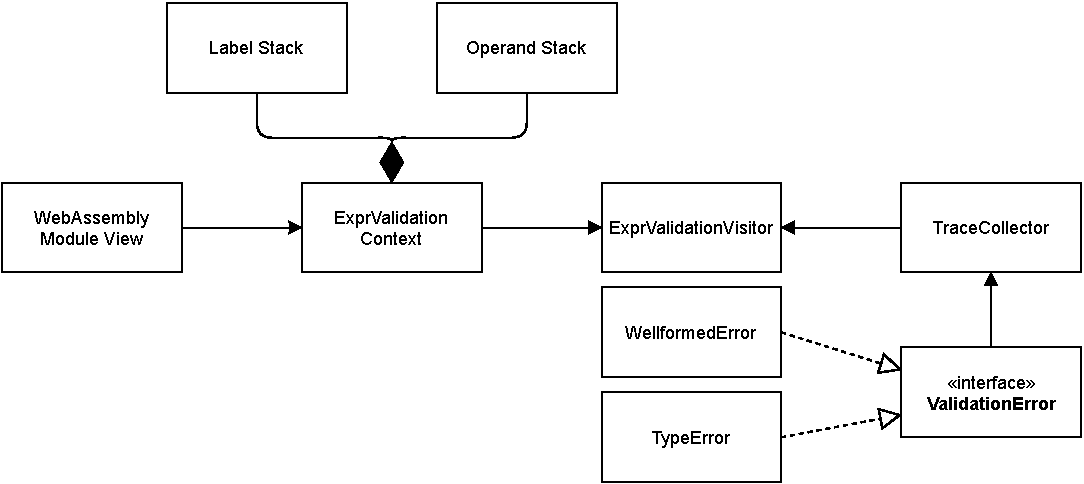
\includegraphics[width=\textwidth]{Images/sablewasm-validation.pdf}
  \caption{SableWasm validation pass}
  \label{fig:sablewasm-validation}
\end{figure}

WebAssembly specification defines a  detailed static validation rule both for well-formedness and type-soundness. Similar to the parser framework, we implement our validation pass as close to the specification as possible. If there are changes to the specification in the future, we can adopt them with minimal effort. The validation pass implementation consists of three parts: the validation context and validation visitor, implementing context and rules in the specification accordingly, and the trace collector used to recover the validation error site.  In figure~\ref{fig:sablewasm-validation}, we present an illustration of the validation pass in SableWasm. Later in the section, we will give a brief introduction to each of the components. The detailed validation rule, both well-formedness and type-soundness, are listed in the WebAssembly introduction paper \cite{10.1145/3062341.3062363}, and a separate paper that focuses on validation \cite{10.1145/3167082}. Note that these two papers only present the validation rules for the minimum viable product (MVP) WebAssembly, and each extension may modify the specification.  The additional validation rules introduced by the extensions adopted by SableWasm are relatively trivial. Hence, we will not give a detailed description, and one should consult the extension proposals for detailed information. 

\paragraph{Validation Context}
Validation context implements the contexts defined in the WebAssembly specification. It provides an easy way for the validation visitor to access the WebAssembly entities' declarations. The validation context itself does not perform any error signalling. The validation context also manages the operand stack and the label stack. The operand stack stores the type information gathered from the instruction within the expression while the label stack keeps track of the signatures of the control flow structures. The operand stack also records the requirements generated from a $\epsilon$ stack and checks if there are contradictions among them. 

\paragraph{Validation Visitor}
The validation visitor is the core driver part of the validation pass. It implements all the validation rules for each instruction and derives from the visitor template. In the current state of implementation, the design of the validation visitor is not modular, and if there are additional instructions add to the project later, direct modification is required. The validation visitor also handles all the error signalling. However, it does not construct the error objects by itself. The task is deferred to the trace collector. For most of the instructions, the validation rule is quite simple, involves only poping and pushing values to the operand stack. Currently, the validation visitor will stop at the first error it encounters due to the design of the WebAssembly validation rules. 

\paragraph{Trace Collector}
The last part of the validation pass implementation is the trace collector. It locates the position of the instruction that currently undergoes validation. It first keeps track of the section where the instruction lives with an enumeration and uses a stack to track how to locate it. Every time the validation visitor enters a nested construct such as \texttt{if}, \texttt{block} or \texttt{loop}, it pushes the construct to the site stack, and pop when nested expression finish validation. If the validation visitor locates an error, the trace collector will build the error by moving the trace stack into the error object.

In this section, we present the validation pass implementation in SableWasm. In the next section, we will perform some experiment benchmarks on the system's performance in terms of execution speed and memory footprint. 

\section{Performance Evaluation}

This section presents the performance benchmark comparison between the SableWasm parser frontend and the WebAssembly binary toolkit (WABT) offered by the WebAssembly community group. The benchmarks focus on both the execution time and memory footprint. We will first present the benchmark setup and then evaluate the data collected from the experiment. 

\begin{figure}
  \centering
  \begin{subfigure}[t]{0.87\textwidth}
    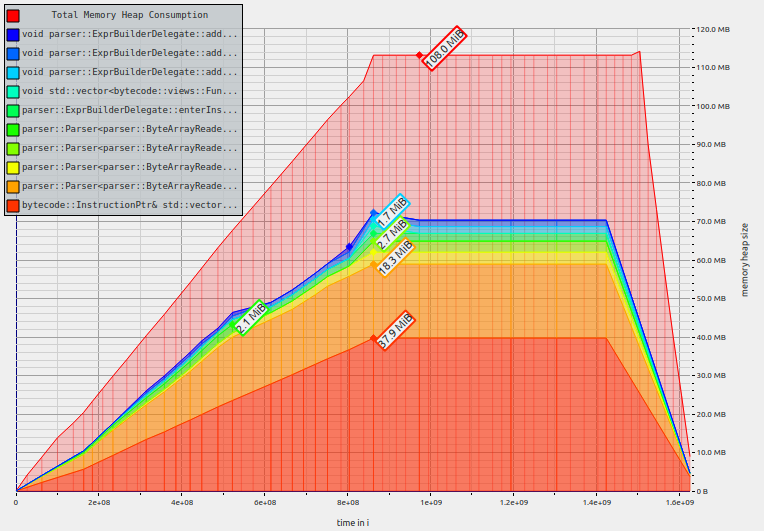
\includegraphics[width=\textwidth]{Images/sablewasm-validate-memory.png}
	\caption{SableWasm}\label{fig:sablewasm-eval-memory-sablewasm}		
  \end{subfigure}
  \begin{subfigure}[t]{0.87\textwidth}
    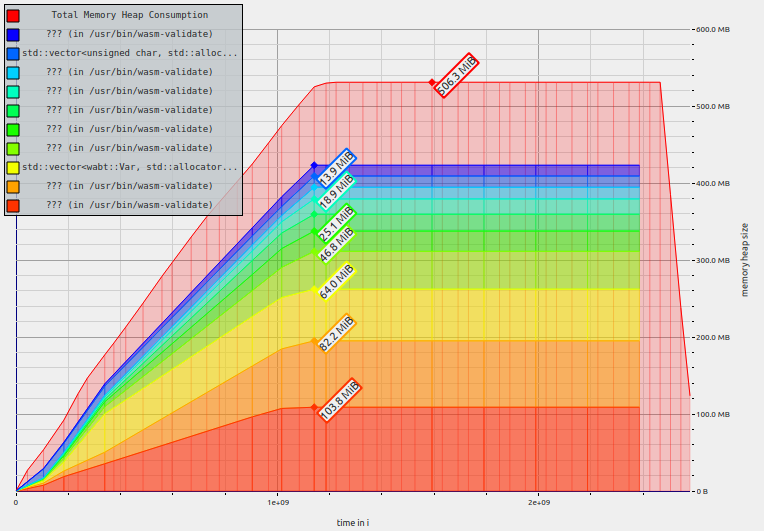
\includegraphics[width=\textwidth]{Images/wabt-validate-memory.png}
	\caption{WABT}\label{fig:sablewasm-eval-memory-wabt}		
  \end{subfigure}
  \caption{Frontend memory footprint comparison}
  \label{fig:sablewasm-eval-memory}
\end{figure}

\paragraph{Benchmark setup}
Experiments were performed on a server with a six-core Intel Core processor at 3.7 GHz standard clock frequency and an L3 cache of 12MiB. The server runs Ubuntu 18.04 with Linux kernel version 4.15.0 and 32GiB of memory. For the benchmark subject, we choose Pyodide \footnote{Pyodide project: \url{https://github.com/pyodide/pyodide}}, a WebAssembly implementation of Python 3.8. The project has reasonable complexity, and the size of the module is quite significant, which reduces the measurement errors during the benchmark. The WebAssembly binary toolkit (WABT) we used during the benchmark is version 1.0.23, and we perform module validation with its \texttt{wasm-validate} command. This command should parse the WebAssembly module, construct an internal bytecode representation, and perform validation pass over it. This procedure is similar to what we used in the SableWasm frontend. For the execution speed experiment, we time the execution speed with shell builtin \texttt{time} command. We perform ten runs of each implementation in total and then compute the average execution speed. For memory footprint, we use the Massif tool provided by Valgrind \cite{valgrind-paper}. Massif is a heap profiler that collects heap memory usage during programs execution lifetime, which we will use to compare two implementations. 

\paragraph{Benchmark Result}
We will go over the finding over the execution speed first and then analyze the memory footprint. Table~\ref{tab:frontend-benmark-time} gives the result of the execution speed benchmark. The data is relatively consistent over a total of ten runs, where the SableWasm frontend achieves around 1.5x to 1.7x speedup compared to \texttt{wasm-validated} provided by WABT. On average, the SableWasm frontend is 1.6x times faster than WABT's implementation.

% Table generated by Excel2LaTeX from sheet 'Sheet1'
\begin{table}[htbp]
  \centering
    \begin{tabular}{lrrr}
    \toprule
    \textbf{Run} & \multicolumn{1}{l}{\textbf{SableWasm}} & \multicolumn{1}{l}{\textbf{WABT}} & \multicolumn{1}{l}{\textbf{Speedup}} \\
    \midrule
    \rowcolor[rgb]{ .851,  .851,  .851} Run \#1 & 0.311 & 0.523 & 1.682 \\
    Run \#2 & 0.308 & 0.511 & 1.659 \\
    \rowcolor[rgb]{ .851,  .851,  .851} Run \#3 & 0.307 & 0.511 & 1.664 \\
    Run \#4 & 0.329 & 0.513 & 1.559 \\
    \rowcolor[rgb]{ .851,  .851,  .851} Run \#5 & 0.336 & 0.520 & 1.548 \\
    Run \#6 & 0.317 & 0.534 & 1.685 \\
    \rowcolor[rgb]{ .851,  .851,  .851} Run \#7 & 0.315 & 0.518 & 1.644 \\
    Run \#8 & 0.335 & 0.522 & 1.558 \\
    \rowcolor[rgb]{ .851,  .851,  .851} Run \#9 & 0.311 & 0.513 & 1.650 \\
    Run \#10 & 0.335 & 0.574 & 1.713 \\
    \rowcolor[rgb]{ .851,  .851,  .851} Average & 0.320 & 0.524 & 1.635 \\
    \bottomrule
    \end{tabular}%
  \caption{Frontend execution speed comparison}
  \label{tab:frontend-benmark-time}%
\end{table}%


On the topic of memory footprint, figure~\ref{fig:sablewasm-eval-memory-sablewasm} and figure~\ref{fig:sablewasm-eval-memory-wabt} shows the memory consumption trace for SableWasm and WABT, respectively. As we can see from the figures, SableWasm consumes approximately 108MiB at peak while WABT uses around 506MiB, suggesting a 4.6x reduction in memory footprint. More specifically, SableWasm spends about 38MiB for bytecode representation, and WABT takes roughly 82MiB, indicating a 2.1x reduction for bytecode representation only. Overall the SableWasm frontend implementation performs better than SableWasm in both terms of execution speed and memory consumption. SableWasm is a static compiler that will only perform parsing and validation at compile-time and does not affect overall execution time for emitted executables. If in the future, one would like to implement a just-in-time (JIT) style compiler, SableWasm parsing and validation frontend can effectively improve the response time of the JIT compiler. 

We visit the design and implementation of the SableWasm frontend, which takes care of parsing, validating and construct bytecode representation in this chapter. In the next chapter, we will move to the next phase in the SableWasm compilation pipeline, the middle-level intermediate representation.